\documentclass[a4paper,12pt]{mwart}
\usepackage[MeX]{polski}
\usepackage[utf8]{inputenc}
\usepackage{indentfirst}
\usepackage{hyperref}
\usepackage{color}
\usepackage{amsmath}
\usepackage{float}

% reset numerowania sekcji w częściach
\usepackage{chngcntr}
\counterwithin*{section}{part}

% zagnieżdżone numerowanie list
\usepackage{enumitem}

\usepackage{tikz}
\usetikzlibrary{arrows,positioning,automata}
\tikzset{>=stealth',shorten >=1pt,auto,thick,main node/.style={circle,fill=blue!30,draw,minimum size=1cm,inner sep=0pt,font=\sffamily\Large\bfseries},wordnet/.style={draw=none,fill=none,inner sep=0pt},edge/.style={thick,double}}

\frenchspacing

\title{
    Grafy i~Sieci \\
    sprawozdania
}
\author{
    Łukasz~Jędrzejewski
    \and
    Igor~Rodzik
}

\date{}

\begin{document}

\maketitle

\part{Sprawozdanie 1}

\section{Temat projektu}

Graf skierowany $G=(V,E)$ jest częściowo spójny, jeśli dla każdych dwóch
wierzchołków $u$ i $v$ z $V$ istnieje ścieżka $u \to v$ lub $v \to u$. Należy
zaimplementować algorytm sprawdzania, czy dany graf $G$ jest częściowo spójny.

\section{Opis merytoryczny zadania}

Naszym zadaniem jest implementacja algorytmu, który ma~sprawdzić, czy podany
graf skierowany jest częściowo spójny.

\subsection{Definicje}

\begin{description}
\item[Ścieżka] trasa, w~której krawędzie nie powtarzają się.
\item[Trasa] ciąg wierzchołków (gdy graf nie jest multigrafem) lub ciąg
  postaci $(v_1,e_1,v_2,e_2,\ldots, v_{n-1}, e_{n-1}, v_n)$.
\item[Multigraf] graf, dla którego dopuszczamy wielokrotne krawędzie między
  dwoma wierzchołkami oraz pętle.
\item[Pętla] krawędź, której końcami jest ten sam wierzchołek.
\item[Graf częściowo spójny] graf, w~którym między każdą parą wierzchołków
  istnieje ścieżka co~najmniej w~jedną stronę.
\item[Listy sąsiedztwa] sposób prezentacji grafu, w którym każdy wierzchołek ma
	przypisaną listę wierzchołków, do których poprowadzona jest krawędź z tego
	wierzchołka.
\end{description}

\subsection{Założenia}

\begin{enumerate}
\item Rozpatrywany graf jest spójny.
\end{enumerate}

\section{Opis wykorzystywanego algorytmu}

W~algorytmie zamierzamy wykorzystać algorytm przeglądania grafu w~głąb lub
wszerz. Algorytm zarządzałby dwiema kolekcjami wierzchołków -- zbiorem
wierzchołków $V1$, które stanowią podgraf częściowo spójny (na~początku zbiór
pusty) oraz wierzchołkami niesprawdzonymi $V2$ wejściowego grafu (na~początku
wszystkie wierzchołki). Następnie powtarzalibyśmy przechodzenie grafu
pobierając pierwszy wierzchołek z~$V2$. Dla wykonanego przejścia należy
sprawdzić, czy wszystkie odwiedzone wierzchołki zawierają się w~zbiorze $V1$.
Jeśli nie, oznacza to, że~graf nie jest częściowo spójny (ponieważ
z~wierzchołków z~$V1$ nie dotarliśmy do~bieżącego wierzchołka, więc z~tego
wierzchołka musimy osiągnąć wszystkie wierzchołki z~$V1$). Jeśli tak, to~należy
powtórzyć krok, dodając do~$V1$ odwiedzone wierzchołki, do~momentu, gdy zbiór
$V1$, będzie stanowił wszystkie wierzchołki wejściowego grafu, lub nie
osiągniemy odwiedzonych do~tej pory wierzchołków z~$V1$.

\section{Literatura}

\noindent Cormen, Thomas H.; Leiserson, Charles E.; Rivest, Ronald L.; Stein,
\emph{Wprowadzenie do~algorytmów}.

\newpage

\part{Sprawozdanie 2}

\section{Algorytmy}

\subsection{Z~definicji}
\label{sec:from-definion-alg}

Dla każdej pary wierzchołków $(v, u)$ grafu sprawdź, czy można osiągnąć
wierzchołek $u$ uruchamiając procedurę \emph{DFS} z~$v$ lub odwrotnie.

\subsection{Bazujący na~silnie spójnych składowych}

Idea kolejnego algorytmu polega na~wyznaczeniu wszystkich silnie spójnych
składowych grafu. Następnie każdą silnie spójną składową zastępujemy
pojedynczym wierzchołkiem. Składowe łączymy krawędzią, jeśli istnieje krawędź
między wierzchołkami należącymi do~składowych. Na~tak zminimalizowanym grafie,
uruchamiamy algorytm sprawdzający z~sekcji~\ref{sec:from-definion-alg}
lub~\ref{sec:multiple-dfs}, czy graf jest częściowo spójny.

% TODO: przykład transformacji?

\subsubsection{Wyznaczenie silnie spójnych składowych}

Jednym z~algorytmów wyznaczających silnie spójne składowe grafu to~algorytm
\textbf{Kosaraju}. Wykorzystuje on~dwa przejścia w~głąb oraz transpozycję
grafu.

Graf \textbf{transponowany} $G^T$ to~graf, w~którym krawędzie są~odwrócone.

Algorytm zaś wygląda następująco:

\begin{enumerate}
\item\label{sec:kosaraju-alg-1-pt} Wyznaczamy listę wierzchołków w~kolejności
  przetworzenia wierzchołków grafu algorytmem DFS, czyli odwrotną
  do~posortowania topologicznego.
\item\label{sec:kosaraju-alg-2-pt} Wykonujemy algorytm DFS dla grafu
  transponowanego, dla każdego wierzchołka
  z~punktu~\ref{sec:kosaraju-alg-1-pt}. Każde otrzymane drzewo DFS, zawiera
  wierzchołki należące do~jednej silnie spójnej składowej.
\end{enumerate}

W~punkcie~\ref{sec:kosaraju-alg-1-pt} ważne jest, aby procedurą DFS odwiedzić
wszystkie wierzchołki. W~ten sposób otrzymamy las drzew DFS.\@ Przechodząc
każde drzewo w~kolejności \emph{post-order} (najpierw podrzewa, na~koniec
węzeł), otrzymamy kolejność odwiedzania wierzchołków wymaganą w~kolejnym kroku.

Krok~\ref{sec:kosaraju-alg-2-pt} algorytmu wykorzystuje własność grafu
transponowanego taką, że~posiada on~identyczne silnie spójne składowe, jak graf
pierwotny. Dodatkowo odwiedzone wierzchołki we~wcześniejszych wywołaniach DFS
powinny być pomijane. Innymi słowy, używamy tego samego zbioru wierzchołków
odwiedzonych dla wszystkich wywołań DFS.

\subsection{Z~wielokrotnym DFS}
\label{sec:multiple-dfs}

Ostatni algorytm opiera się na~wielokrotnym przechodzeniu grafu.

Rozpoczynamy z~listą wierzchołków do~odwiedzenia $toVisit$ oraz pustym zbiorem
wierzchołków odwiedzonych $visited$. Dopóki lista $toVisit$ nie jest pusta:
\begin{enumerate}
\item pobierz pierwszy wierzchołek $v$ z~listy $toVisit$,
\item dla $v$ wywołaj $DFS$,
\item\label{item:multiple-dfs:cond} sprawdź, czy wszystkie odwiedzone
  wierzchołki w~$DFS(v)$ są~w~zbiorze $visited$,
\begin{enumerate}[label*=\arabic*.]
\item jeśli tak, to~usuń z~listy $toVisit$ odwiedzone wierzchołki w~$DFS(v)$,
  a~do~zbioru $visited$ przypisz wierzchołki odwiedzone w~$DFS(v)$,
\item w~przeciwnym przypadku, graf nie jest częściowo spójny.
\end{enumerate}
\end{enumerate}

Intuicja za~punktem~\ref{item:multiple-dfs:cond}, opiera się na~tym,
że~w~pewnym kroku algorytmu, wszystkie wierzchołki w~zbiorze $visited$ stanowią
podgraf częściowo spójny. Wykonując więc DFS na~pierwszym wierzchołku $v$
z~listy $toVisit$, musimy odwiedzić wszystkie wierzchołki z~$visited$. Jeśli
tak się nie stanie, to~graf okaże się nieczęściowo spójny. Wynika to~z~tego,
że~skoro $v$ nie jest osiągalny z~żadnego wierzchołka z~$visited$, to~wszystkie
wierzchołki z~$visited$ muszą być osiągalne przez $v$.

Doprecyzowania wymaga jeszcze kolejność wierzchołków w~liście $toVisit$.
Mianowicie, należy je~przetwarzać w~kolejności odwrotnej do~posortowania
topologicznego wierzchołków. Zapobiega to~przypadkom, że~kilka podgrafów, jest
osiągalnych z~pewnego wierzchołka, mimo że~żadne wierzchołki z~podgrafów nie
są~wzajemnie osiągalne. Jako przykład można rozważyć graf:

\begin{figure}[H]
  \centering
  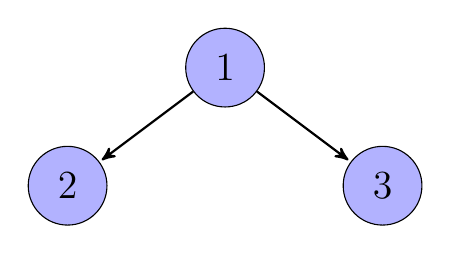
\begin{tikzpicture}
    \node[main node, on grid] (v1) {$1$};
    \node[main node, on grid] (v2) [below right = 1.5cm and -2cm of v1] {$2$};
    \node[main node, on grid] (v3) [below right = 1.5cm and 2cm of v1] {$3$};
    \path[edge] (v1) edge [->] node {} (v2);
    \path[edge] (v1) edge [->] node {} (v3);
  \end{tikzpicture}
\end{figure}

Rozpoczynając od~$1$, wszystkie wierzchołki zostałyby odwiedzone, mimo że~nie
istnieje ścieżka $2 \to 3$ lub $3 \to 2$, więc graf zostałby niepoprawnie
sklasyfikowany jako częściowo spójny.

\section{Struktury danych}

Graf został przedstawiony w naszej aplikacji jako listy sąsiedztwa. Wierzchołki
są oznaczone liczbami całkowitymi. Krawędź przedstawiona została jako para
wierzchołków. Na potrzeby projektu powstała również lista grafów, która służy do
przechowywania grafów utworzonych ręcznie na potrzeby testów jednostkowych oraz
prezentacji możliwości algorytmu w interfejsie użytkownika. Dostępne są również
lista przechowująca wszystkie wierzchołki grafu i analogiczna lista
przechowująca krawędzie. Wynik algorytmu przechowywany jest wraz z grafem w
osobnej strukturze co ma na celu uproszczenie implementacji interfejsu
użytkownika.

\section{Projekt testów}

Obydwa algorytmy przetestujemy na~kilku zdefiniowanych przez nas szczególnych
przypadkach grafów częściowo spójnych, jak i~nie.

Dodatkowo zamierzamy zaimplementować generatory grafów częściowo spójnych i~nie
posiadających tej własności, w~celu sprawdzenia poprawności działania
na~losowych grafach. Wytworzony generator posłuży nam także do~generacji
większych grafów oraz weryfikacji złożoności czasowych algorytmów.

\section{Założenia programu}

\end{document}

%%% Local Variables:
%%% mode: latex
%%% TeX-master: t
%%% End:
